\documentclass[tikz]{standalone}
\usepackage{pgfplots}
\pgfplotsset{compat=1.15}
\usepackage{mathrsfs}
\usetikzlibrary{arrows,calc}
\usepackage{tkz-euclide}

\usepackage{fp}
\pagestyle{empty}

\definecolor{AngleClr}{rgb}{0,0.39215686274509803,0}
\definecolor{ShapeClr}{rgb}{0.6,0.2,0}

\begin{document}

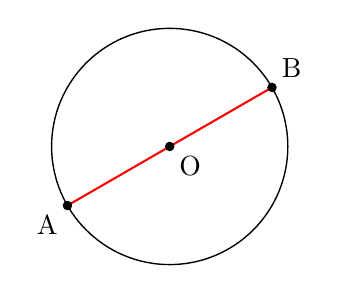
\begin{tikzpicture}[scale=.75]
\tkzSetUpLine[line width=1pt,color=black]
\tkzSetUpPoint[fill=black]

\tkzDefPoints{0/0/O,2/0/X}

\tkzDefPoint(30:2){B}
\tkzDefPoint(-150:2){A}

\tkzDrawSegments[line width=0.75pt,color=red](A,B)

\tkzDrawCircle[color=black,line width=0.5pt](O,X)

\tkzDrawPoints[size=3](A,B,O)

\tkzLabelPoint[below left](A){$\rm A$}
\tkzLabelPoint[above right](B){$\rm B$}
\tkzLabelPoint[below right](O){$\rm O$}


\end{tikzpicture}

\end{document}
